\documentclass{article}

\usepackage{enumitem}
\usepackage{fancyhdr}
\usepackage{listings}
\usepackage{graphicx}
\usepackage{color}

\usepackage[lastexercise, noanswer]{exercise}   %add in noanswer
% for exercise 
\def\AnswerName{Solution to Exercise}

\definecolor{dkgreen}{rgb}{0,0.6,0}
\definecolor{gray}{rgb}{0.5,0.5,0.5}
\definecolor{mauve}{rgb}{0.58,0,0.82}


\lstset{frame=tb,
  language=Haskell,
  aboveskip=3mm,
  belowskip=3mm,
  showstringspaces=false,
  columns=flexible,
  basicstyle={\small\ttfamily},
  numbers=none,
  numberstyle=\tiny\color{gray},
  keywordstyle=\color{blue},
  commentstyle=\color{dkgreen},
  stringstyle=\color{mauve},
  breaklines=true,
  breakatwhitespace=true,
  tabsize=3
  }
%% Change this for title information 
\newcommand\ExTitle{Types and Classes \ }

\newcommand\fullExTitle{Exercises \\ \ExTitle }
\newcommand\footerExTitle{\ExTitle -\  Exercises  and Solutions}

\pagestyle{fancy}
\fancyhead{} % clear all header fields
\renewcommand{\headrulewidth}{0pt} % no line in header area
\fancyfoot{} % clear all footer fields
\fancyfoot[LE,RO]{\thepage}           % page number in "outer" position of footer line
\fancyfoot[RE,LO]{\footerExTitle} % other info in "inner" position of footer line

%\usepackage[mathrm,colour,cntbysection]
  
\begin{document}
\begin{Huge}
	\begin{center}
	\fullExTitle
	\end{center}
\end{Huge}

\begin{Exercise} 
%
	
  What are the types of the following values?  \\
\begin{lstlisting}
    ['a', 'b', 'c']
    ('a', 'b', 'c')
    [(False, '0'), (True, '1')]
    (['1', '0'], ['0', '1'])
    [tail, init, reverse]	
\end{lstlisting}
   Use GHCi (:t) to check your answers. 
\end{Exercise}
\begin{Answer}
\begin{lstlisting}
    ['a', 'b', 'c']  ----> type ----> [Char]
    ('a', 'b', 'c')  ----> type ----> (Char,Char, Char)
    [(False, '0'), (True, '1')]  ----> type ---->  [(Bool. Char)]
    (['1', '0'], ['0', '1'])   ----> type ----> ([Char], [Char])
    [tail, init, reverse]	----> type ----> [ [a]-> [a] ]
\end{lstlisting}
\end{Answer}



\begin{Exercise}
   Write down definitions that have the following types. It does not matter that the definitions actually do as long as they are type correct:
\begin{lstlisting}
    bools :: [Bool]
    nums :: [[Int]]
    add :: Int -> Int -> Int-> Int
    copy :: a -> (a,a)
    apply :: (a -> b) -> a -> b	
\end{lstlisting}
Check your answers using GHCi. You can do this using a script or by using the let construct: \\
\begin{center}
	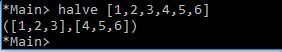
\includegraphics[width=8cm]{img/01.jpg}
\end{center}
\end{Exercise}
\begin{Answer}
Using script 
\begin{lstlisting}
  bools :: [Bool]
  bools = [True, False]
  nums :: [[Int]]
  nums = [ [1,2,3], [2,3,4]]
  add :: Int -> Int -> Int-> Int
  add x y z= x + y + z
  copy :: a -> (a,a)
  copy x = (x, x)
  apply  :: (a->b) ->  a -> b
  apply double x  = double x
\end{lstlisting}
\end{Answer}



\begin{Exercise}
What are the types of the following functions? \\
\begin{lstlisting}
    second xs = head (tail xs)
    swap (x,y) = (y,x)
    pair x y = (x,y)
    double x = x*2
    pallindrome xs = reverse xs == xs
    twice f x = f (f x)
\end{lstlisting}
The easiest way to check this is to use the \emph{:t} at the console. 
You can also check this by putting these in a script with the type. If they are not consistent, you will get an error when you run/load the script. \\
Also, take care to include the necessary class constraints (e.g. Eq a $=>$ when you are testing for equality)if the functions are defined using overloaded operators. 
\end{Exercise}
\begin{Answer}
\begin{lstlisting}
  copy :: a -> (a,a)
  copy x = (x, x)
  second :: [a] -> a
  second xs = head (tail xs)
  swap :: (a,b) -> (b,a)
  swap (x,y) = (y,x)
  pair :: a -> b-> (a,b)
  pair x y = (x,y)
  double ::Num a => a -> a
  double x = x +x
  pallindrome :: Eq a =>  [a] -> Bool
  pallindrome xs = reverse xs == xs
  twice :: (a->a) -> a -> a
  twice f x = f (f x)

\end{lstlisting}
\end{Answer}
% Uncomment this for the Answers
% \newpage
% \begin{Huge}
% \begin{center}
% Solutions
% \end{center}
% \end{Huge}
% \shipoutAnswer

\end{document}
